\documentclass[10pt,a4paper]{article}
\usepackage[margin=22mm]{geometry}
\usepackage{fontspec,graphicx,booktabs,array}
\usepackage[french]{babel}
\setmainfont{Cambria}
\setsansfont{Calibri}
\pagestyle{plain}
\setlength{\parindent}{0pt}
\setlength{\parskip}{5pt}
\setlength{\emergencystretch}{2em}
\raggedbottom
\begin{document}
{\sffamily\LARGE\bfseries TP Frugal AI}\par
{\large Trinh Cédric}\par
\smallskip\hrule\medskip

\section*{\sffamily Partie 1 — Multiplier deux matrices}

\subsection*{\sffamily Q1–2 · Machine et puissance au repos}

Le poste de la salle est un \textbf{i7-12700} avec 8 cœurs P à deux threads et 4 cœurs E à un thread, soit \textbf{12 cœurs et 20 threads}. Il dispose de 15 Gio de RAM utilisable, d’AVX2 et de FMA. En FP32, un registre AVX2 contient huit nombres. Le L1 totalise 512 Kio de données et 512 Kio d’instructions. Les 12 Mio de L2 se répartissent en huit caches privés de 1,25 Mio et un cache de 2 Mio partagé par les quatre cœurs E. Les 25 Mio de L3 sont partagés.

\begin{center}\small\setlength{\tabcolsep}{3pt}\renewcommand{\arraystretch}{1.16}

\begin{tabular}{>{\raggedright\arraybackslash}p{\dimexpr 0.130\linewidth-14\tabcolsep*130/1000\relax}>{\raggedright\arraybackslash}p{\dimexpr 0.080\linewidth-14\tabcolsep*80/1000\relax}>{\raggedright\arraybackslash}p{\dimexpr 0.120\linewidth-14\tabcolsep*120/1000\relax}>{\raggedright\arraybackslash}p{\dimexpr 0.120\linewidth-14\tabcolsep*120/1000\relax}>{\raggedright\arraybackslash}p{\dimexpr 0.140\linewidth-14\tabcolsep*140/1000\relax}>{\raggedright\arraybackslash}p{\dimexpr 0.150\linewidth-14\tabcolsep*150/1000\relax}>{\raggedright\arraybackslash}p{\dimexpr 0.160\linewidth-14\tabcolsep*160/1000\relax}}\toprule

\textbf{Situation} & \textbf{Veille} & \textbf{Repos écran éteint} & \textbf{Repos écran allumé} & \textbf{VS Code + Firefox} & \textbf{Ouverture d’un PDF} & \textbf{YouTube sans / avec accélération}\\ \midrule

Puissance à la prise & 1,7 W & 8 W & 16 W & 20 W & pic à 30 W & 28 / 27 W\\

\bottomrule\end{tabular}\end{center}

Au repos, la puissance passe de 8 à 16 W quand l’écran s’allume. Pendant la lecture de la vidéo YouTube, l’accélération matérielle réduit la puissance mesurée de \textbf{28 à 27 W} (environ 4 \%). Le décodage vidéo dédié peut décharger le CPU, ce qui est cohérent avec la baisse observée.

\subsection*{\sffamily Q3–8 · Python, Numba et NumPy}

Les quatre versions calculent le même produit de matrices FP32 de taille \textbf{512 × 512}.

\begin{center}\small\setlength{\tabcolsep}{3pt}\renewcommand{\arraystretch}{1.16}

\begin{tabular}{>{\raggedright\arraybackslash}p{\dimexpr 0.090\linewidth-10\tabcolsep*90/1000\relax}>{\raggedright\arraybackslash}p{\dimexpr 0.190\linewidth-10\tabcolsep*190/1000\relax}>{\raggedright\arraybackslash}p{\dimexpr 0.250\linewidth-10\tabcolsep*250/1000\relax}>{\raggedright\arraybackslash}p{\dimexpr 0.210\linewidth-10\tabcolsep*210/1000\relax}>{\raggedright\arraybackslash}p{\dimexpr 0.260\linewidth-10\tabcolsep*260/1000\relax}}\toprule

\textbf{Q3–5} & \textbf{Trois boucles Python} & \textbf{Produit et somme NumPy dans la boucle} & \textbf{Trois boucles avec Numba} & \textbf{Produit et somme NumPy avec Numba}\\ \midrule

Temps & 27,510 s & 0,480 s & \textbf{0,062 s} & 0,130 s\\

\bottomrule\end{tabular}\end{center}

Déplacer la boucle interne dans NumPy donne un gain de \textbf{57×}. Numba accélère les trois boucles de \textbf{445×}, et la version avec somme NumPy de \textbf{3,69×}. Une fois compilée, la boucle simple évite de construire un vecteur intermédiaire pour chaque case de C.

\textbf{Q6–7.} Les deux figures comparent les mêmes opérations sur deux grilles de tailles. Le débit est exprimé en milliards de produits-accumulations par seconde selon la convention N\textsuperscript{3} du TP. Plus la courbe est haute, plus le calcul est rapide à taille égale.

\noindent\begin{minipage}{\linewidth}\centering

{\sffamily\bfseries Figure 1 — Multiplication en Python pour des tailles multiples de 128}\par

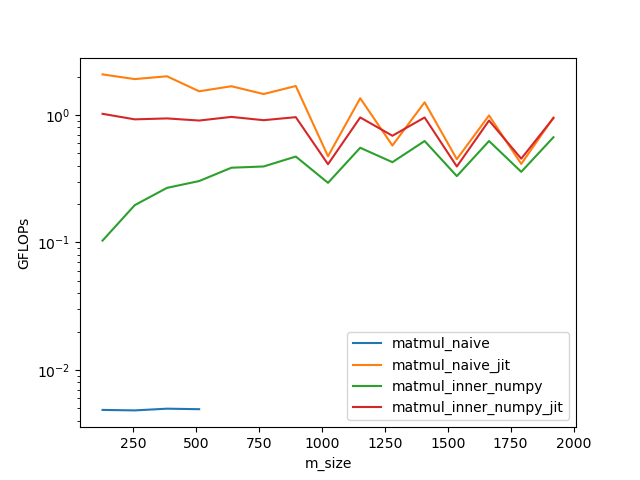
\includegraphics[width=.88\linewidth,height=53mm,keepaspectratio]{6.png}\par

{\small\itshape À N = 1 024, les trois variantes les plus rapides perdent du débit au même endroit. Toutes parcourent B colonne par colonne.\par}\end{minipage}\par

\noindent\begin{minipage}{\linewidth}\centering

{\sffamily\bfseries Figure 2 — Effet du décalage des tailles en Python}\par

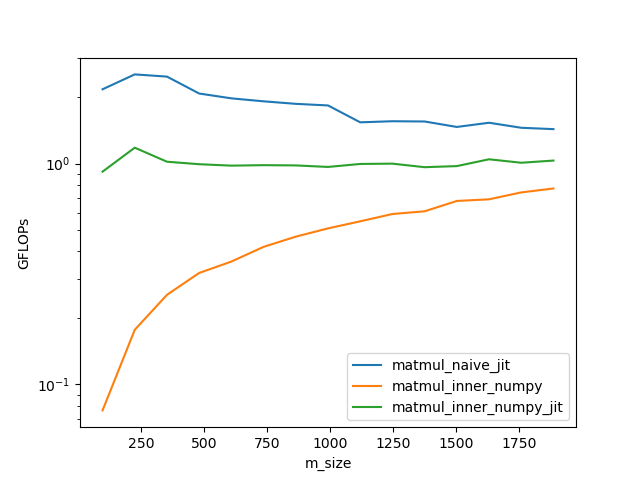
\includegraphics[width=.88\linewidth,height=53mm,keepaspectratio]{7.png}\par

{\small\itshape Pour N = 96, 224, 352, etc., les creux de débit sont moins marqués. Le décalage change l’espacement des lectures de B et peut réduire les conflits de cache.\par}\end{minipage}\par

\textbf{Q8.} Les courbes de \texttt{@}, \texttt{np.matmul} et \texttt{np.dot} se rejoignent autour de 70 GFLOP/s sur les grandes matrices. Les trois utilisent une multiplication matricielle optimisée pour ces tableaux FP32. Les figures Python et C séquentiel comptent \textbf{N\textsuperscript{3}} opérations. Les figures OpenMP et GPU comptent \textbf{2N\textsuperscript{3}} (une multiplication et une addition). Les temps restent directement comparables.

\noindent\begin{minipage}{\linewidth}\centering

{\sffamily\bfseries Figure 3 — Comparaison des trois produits matriciels NumPy}\par

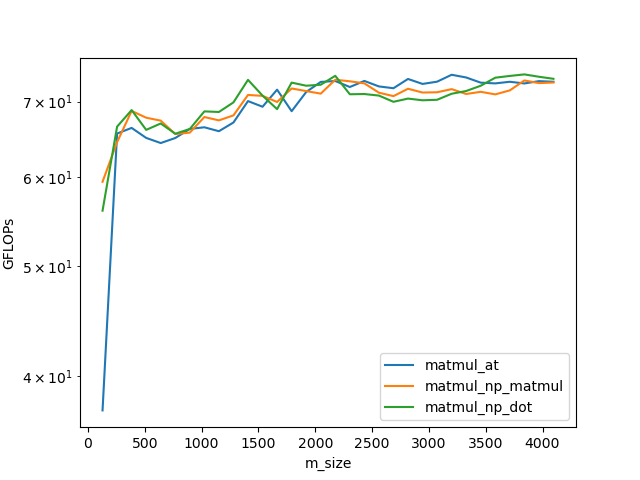
\includegraphics[width=.88\linewidth,height=53mm,keepaspectratio]{8.png}\par

{\small\itshape Les débits de \texttt{@}, \texttt{np.dot} et \texttt{np.matmul} convergent vers le même plateau sur les grandes matrices. Le coût de chaque appel compte surtout sur les petites.\par}\end{minipage}\par

\subsection*{\sffamily Q9–20 · C, accès mémoire et vectorisation}

Temps moyens à \textbf{N = 1 920}, en secondes. La dernière colonne utilise \texttt{-O3 -march=native -funroll-loops -ffast-math}. Les pourcentages ci-dessous comparent chaque version à OpenBLAS mesuré dans le même essai.

\begin{center}\small\setlength{\tabcolsep}{3pt}\renewcommand{\arraystretch}{1.16}

\begin{tabular}{>{\raggedright\arraybackslash}p{\dimexpr 0.270\linewidth-12\tabcolsep*270/1000\relax}>{\raggedright\arraybackslash}p{\dimexpr 0.150\linewidth-12\tabcolsep*150/1000\relax}>{\raggedright\arraybackslash}p{\dimexpr 0.100\linewidth-12\tabcolsep*100/1000\relax}>{\raggedright\arraybackslash}p{\dimexpr 0.100\linewidth-12\tabcolsep*100/1000\relax}>{\raggedright\arraybackslash}p{\dimexpr 0.100\linewidth-12\tabcolsep*100/1000\relax}>{\raggedright\arraybackslash}p{\dimexpr 0.280\linewidth-12\tabcolsep*280/1000\relax}}\toprule

\textbf{Version} & \textbf{Sans option} & \textbf{-O1} & \textbf{-O2} & \textbf{-O3} & \textbf{Toutes les options}\\ \midrule

v1 · trois boucles & 18,386 & 12,243 & \textbf{5,394} & 5,459 & —\\

v2 · accumulateur & 12,948 & \textbf{4,791} & 4,923 & 5,257 & —\\

v3 · transposition de A & 12,093 & 2,958 & 2,887 & 2,936 & \textbf{0,477}\\

v4 · vecteurs de 8 floats & 11,893 & 1,754 & 1,677 & 1,723 & \textbf{0,473}\\

\bottomrule\end{tabular}\end{center}

\textbf{Q9–11.} Sans option, v1 atteint seulement \textbf{0,55 \%} du débit d’OpenBLAS dans la série répétée. Passer à \texttt{-O2} divise le temps par 3,4. \texttt{-O3} apporte peu ici. À la même taille, Numba prend \textbf{8,508 s} en moyenne sur trois passages hors compilation. Le code machine produit par Numba devance le C sans option (18,386 s). Activer les optimisations de GCC inverse le classement (5,394 s avec \texttt{-O2}).

\noindent\begin{minipage}{\linewidth}\centering

{\sffamily\bfseries Figure 4 — Effet d’un accumulateur local en C}\par

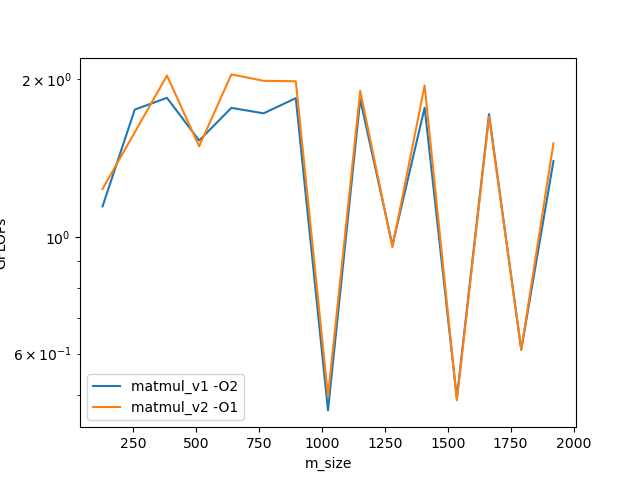
\includegraphics[width=.88\linewidth,height=53mm,keepaspectratio]{q11_13.png}\par

{\small\itshape Les versions avec et sans accumulateur ralentissent toutes deux à N = 1 024 et 1 536. Réduire les écritures dans C conserve le même parcours à grands pas dans A.\par}\end{minipage}\par

\textbf{Q12–13.} v2 accumule chaque produit dans une variable locale et écrit C une seule fois en fin de boucle. Le gain est surtout visible sans optimisation. Avec les meilleurs réglages, le temps passe de 5,39 à 4,79 s. L’accès à une colonne avec un grand pas mémoire reste coûteux.

\textbf{Q14–15.} Le code C stocke les matrices colonne par colonne. Transposer A permet de lire à la suite les valeurs de A et B nécessaires au produit scalaire. Avec \texttt{-O2}, le temps passe de 4,92 à 2,89 s, transposition comprise.

\noindent\begin{minipage}{\linewidth}\centering

{\sffamily\bfseries Figure 5 — Effet des options de compilation après transposition de A}\par

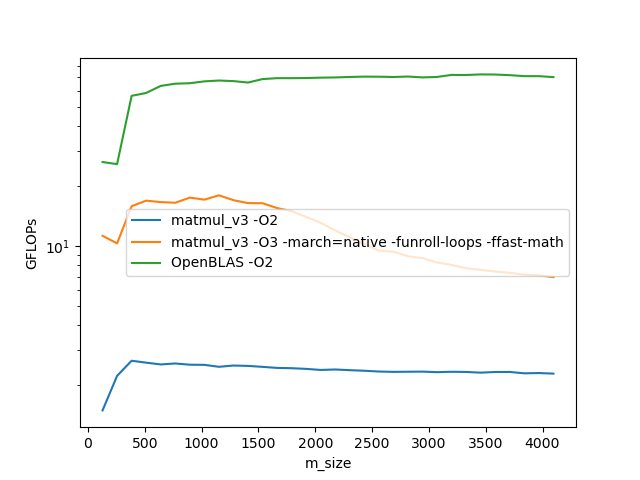
\includegraphics[width=.88\linewidth,height=53mm,keepaspectratio]{q15_17.png}\par

{\small\itshape Le débit de v3 optimisée baisse entre N = 1 152 et 4 096 malgré des lectures contiguës. OpenBLAS maintient mieux son débit en réutilisant les données.\par}\end{minipage}\par

\textbf{Q16–17.} À 1 920, ajouter uniquement \texttt{-march=native} ou \texttt{-funroll-loops} à \texttt{-O3} laisse v3 près de 2,9 s. Avec \texttt{-ffast-math}, le compilateur peut réassocier la somme et le temps descend à \textbf{0,794 s}. Les trois options ensemble donnent \textbf{0,477 s}, soit \textbf{21 \% d’OpenBLAS}. À 4 096, la courbe optimisée tombe à \textbf{7,0} contre \textbf{70,3} pour OpenBLAS. Les deux vecteurs sont contigus, mais chaque case de C exige une nouvelle lecture des deux vecteurs.

\textbf{Q18–20.} v4 charge huit floats de A transposée et huit de B, multiplie les huit paires puis accumule dans huit sommes partielles. À la fin, on additionne ces huit sommes pour obtenir une case de C. Avec \texttt{-O2}, v4 prend 1,68 s contre 2,89 s pour v3. Avec toutes les options, \textbf{0,473 et 0,477 s} sont pratiquement identiques. La vectorisation manuelle apporte peu quand le compilateur vectorise déjà bien la boucle.

\noindent\begin{minipage}{\linewidth}\centering

{\sffamily\bfseries Figure 6 — Vectorisation par groupes de huit valeurs}\par

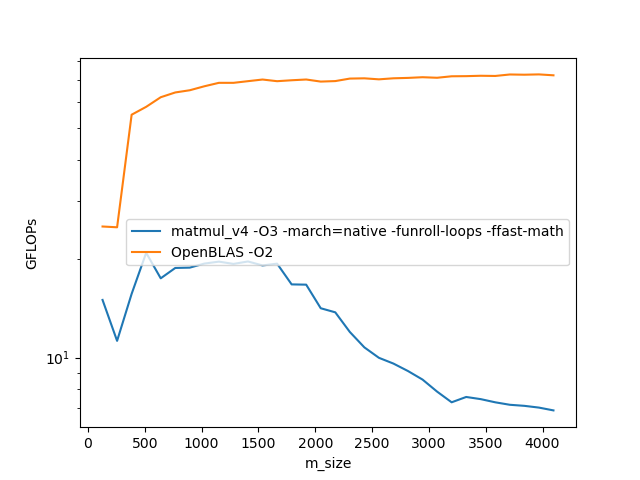
\includegraphics[width=.88\linewidth,height=53mm,keepaspectratio]{q20.png}\par

{\small\itshape Le débit de v4 culmine à N = 512. Quand les matrices grandissent, les relectures de vecteurs pèsent davantage et l’écart avec OpenBLAS se creuse.\par}\end{minipage}\par

\subsection*{\sffamily Q21–27 · Réutiliser les données dans les registres et les caches}

\textbf{Q21–23.} v5 calcule une tuile de C. Un vecteur de A sert à plusieurs colonnes, et un scalaire de B à plusieurs lignes. Les sommes partielles restent dans des registres pendant le parcours de K. À 1 920, v5 prend \textbf{10,58 / 3,61 / 5,22 / 4,76 s} sans option puis avec \texttt{-O1/-O2/-O3}. Avec toutes les options, elle descend à \textbf{0,249 s}, soit \textbf{41 \% d’OpenBLAS}. À 3 840, elle atteint seulement \textbf{10,1} contre \textbf{73,6} pour OpenBLAS. La tuile améliore la réutilisation locale, mais les accès aux grandes matrices restent coûteux.

\noindent\begin{minipage}{\linewidth}\centering

{\sffamily\bfseries Figure 7 — Calcul par tuiles dans les registres}\par

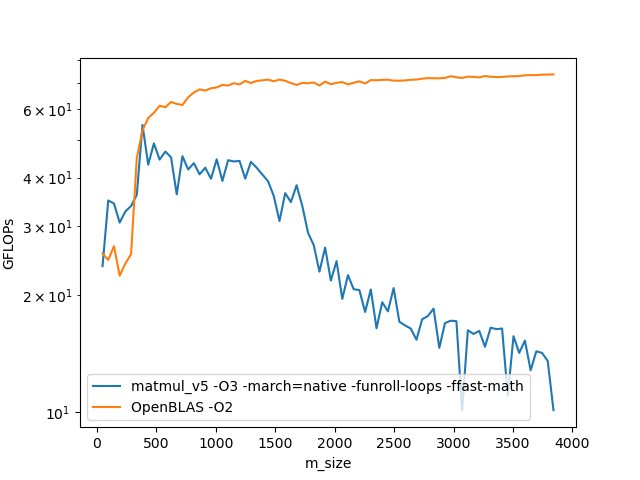
\includegraphics[width=.88\linewidth,height=53mm,keepaspectratio]{q23.png}\par

{\small\itshape Sur les petites matrices, v5 approche le débit d’OpenBLAS. À grande taille, les relectures de A et B d’une tuile à la suivante limitent le gain.\par}\end{minipage}\par

\textbf{Q24.} Une tuile de hauteur H et de largeur W demande \texttt{(H/8) × W} accumulateurs vectoriels, auxquels s’ajoutent les registres des opérandes.

\begin{center}\small\setlength{\tabcolsep}{3pt}\renewcommand{\arraystretch}{1.16}

\begin{tabular}{>{\raggedright\arraybackslash}p{\dimexpr 0.250\linewidth-8\tabcolsep*250/1000\relax}>{\raggedright\arraybackslash}p{\dimexpr 0.250\linewidth-8\tabcolsep*250/1000\relax}>{\raggedright\arraybackslash}p{\dimexpr 0.250\linewidth-8\tabcolsep*250/1000\relax}>{\raggedright\arraybackslash}p{\dimexpr 0.250\linewidth-8\tabcolsep*250/1000\relax}}\toprule

\textbf{Tuile} & \textbf{Accumulateurs} & \textbf{N = 240} & \textbf{N = 1 920}\\ \midrule

8 × 6 & 6 & 0,551 ms & 310 ms\\

16 × 6 & 12 & 0,527 ms & \textbf{242 ms}\\

16 × 8 & 16 & 0,605 ms & 251 ms\\

\bottomrule\end{tabular}\end{center}

À 240, les écarts sont petits devant la dispersion. À 1 920, la tuile \textbf{16 × 6} donne le meilleur temps moyen. Agrandir encore la tuile augmente la pression sur les registres.

\textbf{Q25–27.} v6 découpe aussi M, N et K en blocs. Plusieurs appels au kernel réutilisent alors les mêmes données en cache. Dans la même série à 1 920, v4 prend \textbf{466 ms}, v5 \textbf{228 ms}, v6 \textbf{136 ms}. Parmi les dix découpages testés, \textbf{64/120/480} donne la meilleure moyenne, \textbf{133,4 ± 4,9 ms}, soit \textbf{77 \% d’OpenBLAS}. Le découpage 64/120/240 est proche à 134,9 ms. À 3 840, v6 conserve \textbf{51,4} contre \textbf{73,9} pour OpenBLAS, alors que v5 est à \textbf{10,0}.

\noindent\begin{minipage}{\linewidth}\centering

{\sffamily\bfseries Figure 8 — Effet du découpage en blocs de cache}\par

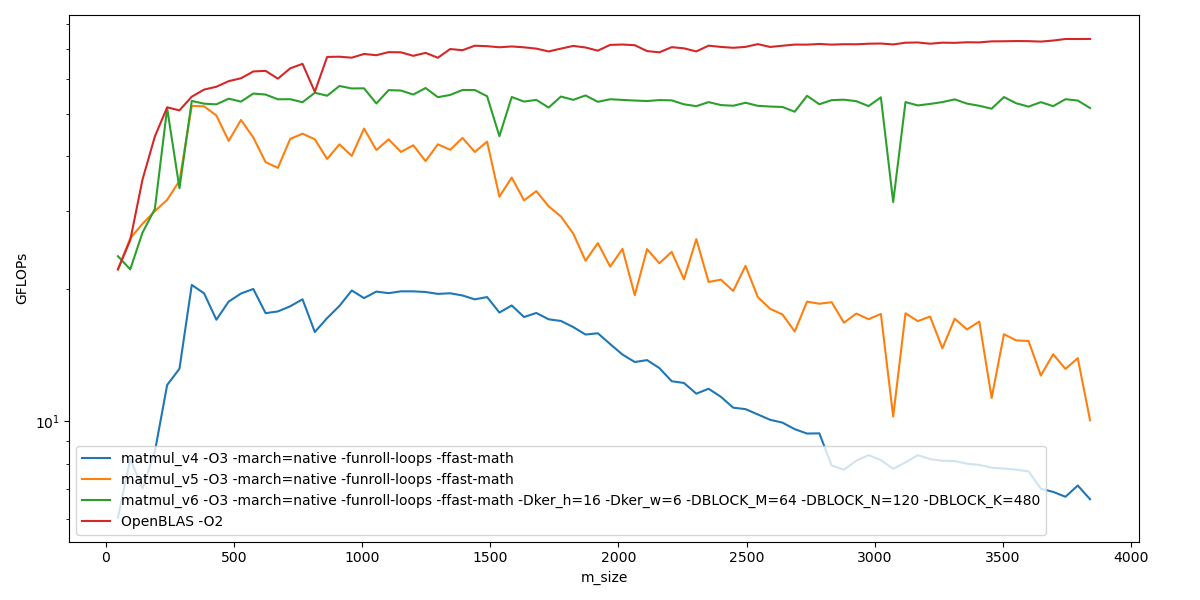
\includegraphics[width=.88\linewidth,height=53mm,keepaspectratio]{q27.png}\par

{\small\itshape À N = 3 840, v6 conserve environ cinq fois le débit de v5. Plusieurs tuiles de C réutilisent les mêmes blocs de A et B en cache.\par}\end{minipage}\par

\subsection*{\sffamily Q28–34 · OpenMP et énergie}

\textbf{Q28–29.} Chaque thread reçoit des blocs distincts de C et garde toutes leurs contributions sur K. Deux threads qui feraient \texttt{C[i,j] += …} en même temps pourraient perdre une contribution. À N = 1 920 et avec deux threads, l’axe M donne \textbf{73,4 ms} contre \textbf{77,3 ms} sur N. Sur M, \texttt{static,1} donne \textbf{66,5 ms}, \texttt{guided,2} \textbf{67,1 ms} et \texttt{dynamic,1} \textbf{69,1 ms}. Le travail est assez régulier pour une répartition statique. Une autre campagne favorise N avec \texttt{static,4}. Le classement varie donc entre les deux séries.

\textbf{Q30–32.} Avec M, \texttt{static,1} et les blocs 64/120/480, le débit passe de \textbf{109 GFLOP/s à 1 thread} à \textbf{444 à 8}, puis \textbf{600 à 20}. À 24 threads il retombe à \textbf{476}. Les deux courbes de speedup se superposent presque parce que les références sont très proches \textbf{(130,54 ms sans OpenMP et 129,96 ms avec un thread)}. À 20 threads, les gains correspondants sont \textbf{5,53× et 5,51×}.

\noindent\begin{minipage}{\linewidth}\centering

{\sffamily\bfseries Figure 9 — Débit selon le nombre de threads OpenMP}\par

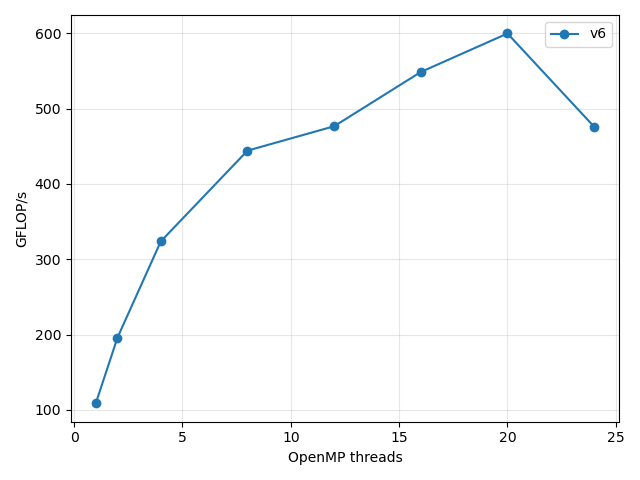
\includegraphics[width=.88\linewidth,height=53mm,keepaspectratio]{openmp_results/q30.png}\par

{\small\itshape À N = 1 920, le débit de v6 quadruple entre 1 et 8 threads, puis progresse plus lentement jusqu’à 20. À 24 threads, la demande dépasse les 20 threads matériels et le débit recule.\par}\end{minipage}\par

\noindent\begin{minipage}{\linewidth}\centering

{\sffamily\bfseries Figure 10 — Accélération par rapport au calcul sur un thread}\par

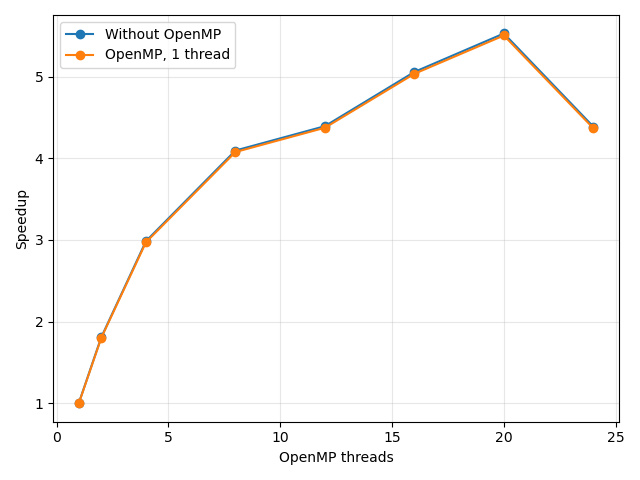
\includegraphics[width=.88\linewidth,height=53mm,keepaspectratio]{openmp_results/q32.png}\par

{\small\itshape À 20 threads, v6 va environ 5,5 fois plus vite. Les courbes se superposent car les deux références, sans OpenMP et avec OpenMP à un thread, prennent presque le même temps.\par}\end{minipage}\par

\textbf{Q33.} Si la puissance double, \texttt{E(12)/E(1) = 2 × t(12)/t(1)}. Avec une répartition des blocs de v6 sur N en \texttt{static,4} et des blocs de 64/120/240, le rapport estimé vaut \textbf{0,645 pour v6} et \textbf{0,647 pour OpenBLAS}. Cela représente une économie d’environ \textbf{35 \% d’énergie} dans les deux cas. Le gain de temps compense le doublement supposé de la puissance. En répartissant les blocs sur M avec le réglage \texttt{static,1} et des blocs de 64/120/480, le même calcul donne \textbf{0,457 pour v6}.

\textbf{Q34.} À \textbf{N = 9 600}, le wattmètre donne 20 W au repos. En charge, les relevés sont les suivants.

\begin{center}\small\setlength{\tabcolsep}{3pt}\renewcommand{\arraystretch}{1.16}

\begin{tabular}{>{\raggedright\arraybackslash}p{\dimexpr 0.240\linewidth-18\tabcolsep*240/1000\relax}>{\raggedright\arraybackslash}p{\dimexpr 0.095\linewidth-18\tabcolsep*95/1000\relax}>{\raggedright\arraybackslash}p{\dimexpr 0.095\linewidth-18\tabcolsep*95/1000\relax}>{\raggedright\arraybackslash}p{\dimexpr 0.095\linewidth-18\tabcolsep*95/1000\relax}>{\raggedright\arraybackslash}p{\dimexpr 0.095\linewidth-18\tabcolsep*95/1000\relax}>{\raggedright\arraybackslash}p{\dimexpr 0.095\linewidth-18\tabcolsep*95/1000\relax}>{\raggedright\arraybackslash}p{\dimexpr 0.095\linewidth-18\tabcolsep*95/1000\relax}>{\raggedright\arraybackslash}p{\dimexpr 0.095\linewidth-18\tabcolsep*95/1000\relax}>{\raggedright\arraybackslash}p{\dimexpr 0.095\linewidth-18\tabcolsep*95/1000\relax}}\toprule

\textbf{Threads} & \textbf{1} & \textbf{2} & \textbf{4} & \textbf{8} & \textbf{12} & \textbf{16} & \textbf{20} & \textbf{24}\\ \midrule

Puissance (W) & 63 & 86 & 136 & 171 & 170 & 162 & 157 & 166\\

Temps v6 (s) & 19,77 & 10,13 & 6,77 & 5,05 & 4,99 & 4,99 & \textbf{4,70} & 5,08\\

GFLOP/J à la prise & 1,42 & 2,03 & 1,92 & 2,05 & 2,09 & 2,19 & \textbf{2,40} & 2,10\\

\bottomrule\end{tabular}\end{center}

\textbf{20 threads donnent à la fois le meilleur temps et le meilleur rendement.} À 8 threads le poste consomme davantage (171 W contre 157 W) pour un calcul plus lent. Après soustraction des 20 W au repos, le maximum reste à 20 threads, avec \textbf{2,75 GFLOP/J}. Ce calcul associe deux passages à 9 600 sur le même poste et suppose que les watts stabilisés ont été relevés pendant v6.

\subsection*{\sffamily Q35–40 · CPU contre T4}

\textbf{Q35.} À N = 4 096, voici le temps moyen de trois multiplications. Sur le T4, les matrices sont déjà en mémoire GPU et le chronométrage exclut les transferts.

\begin{center}\small\setlength{\tabcolsep}{3pt}\renewcommand{\arraystretch}{1.16}

\begin{tabular}{>{\raggedright\arraybackslash}p{\dimexpr 0.600\linewidth-6\tabcolsep*600/1000\relax}>{\raggedright\arraybackslash}p{\dimexpr 0.200\linewidth-6\tabcolsep*200/1000\relax}>{\raggedright\arraybackslash}p{\dimexpr 0.200\linewidth-6\tabcolsep*200/1000\relax}}\toprule

\textbf{Version} & \textbf{Temps} & \textbf{GFLOP/s}\\ \midrule

OpenBLAS CPU, 1 thread & 971,4 ms & 141\\

OpenBLAS CPU, 8 threads & 160,4 ms & 857\\

cuBLAS T4, FP32 & \textbf{33,3 ms} & \textbf{4 128}\\

CUDA naïf & 3 052,1 ms & 45\\

CUDA par tuiles & 64,8 ms & 2 121\\

GemmEx, entrées FP16 et accumulation FP32 & \textbf{2,77 ms} & \textbf{49 574}\\

\bottomrule\end{tabular}\end{center}

\textbf{Q36.} À 4 096, cuBLAS FP32 est \textbf{29,2×} plus rapide qu’OpenBLAS à un thread et \textbf{4,8×} plus rapide qu’à huit threads. Le T4 est déjà devant à la première taille testée (1 024). La multiplication offre assez de cases indépendantes pour exploiter le parallélisme du GPU à cette taille. À 16 384, il atteint \textbf{4 080 GFLOP/s}, contre \textbf{684} sur CPU.

\noindent\begin{minipage}{\linewidth}\centering

{\sffamily\bfseries Figure 11 — Multiplication FP32 sur le CPU de la salle et le GPU T4}\par

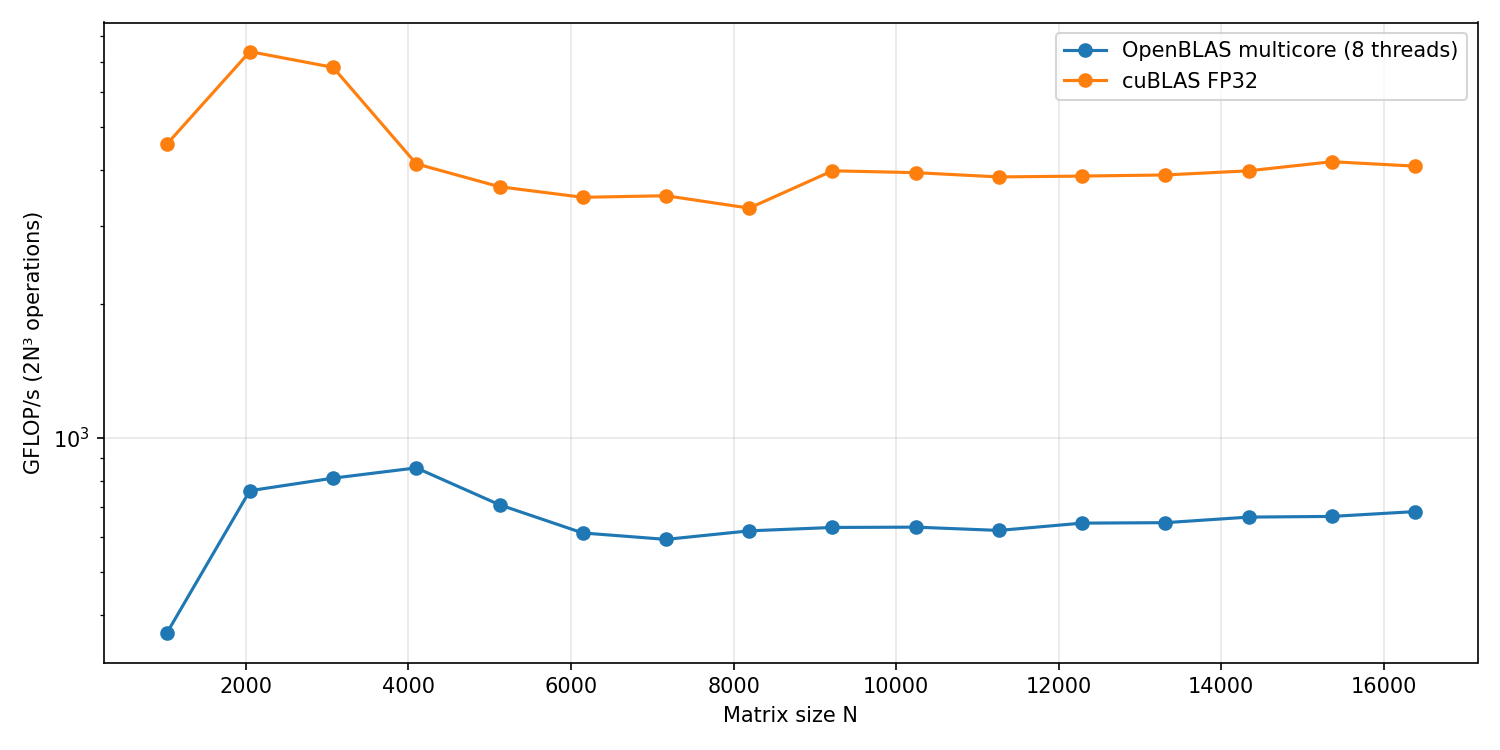
\includegraphics[width=.88\linewidth,height=53mm,keepaspectratio]{gpu_results/q36_cpu_gpu.png}\par

{\small\itshape cuBLAS sur T4 dépasse OpenBLAS sur huit threads dès N = 1 024. Le débit culmine à N = 2 048 sur GPU et à N = 4 096 sur CPU, puis augmente peu avec la taille.\par}\end{minipage}\par

\textbf{Q37.} Avec la puissance turbo maximale publiée par Intel pour le i7-12700 (\textbf{180 W}), le CPU atteint au mieux \textbf{857/180 = 4,76 GFLOP/J}, à 4 096. En supposant une puissance de \textbf{70 W} pour le GPU, le T4 en FP32 atteint \textbf{7 377/70 = 105,4 GFLOP/J}, à 2 048. Le rapport estimé vaut \textbf{22×}. Ces chiffres utilisent une puissance constante sur toute la courbe.

\textbf{Q38.} Chaque thread du kernel naïf calcule une seule case de C et relit deux valeurs à chaque tour sur K. Son meilleur résultat relatif est \textbf{1,09 \% de cuBLAS}, à 4 096. À cette taille, même OpenBLAS sur un seul thread le devance.

\textbf{Q39.} Le kernel par tuiles partage les données d’un bloc et conserve plusieurs sommes en registres. À 4 096, il est \textbf{47×} plus rapide que le naïf et atteint \textbf{51 \% de cuBLAS}. Son meilleur rapport est \textbf{64 \% à 1 024}. Son débit maximal arrive à 2 048, puis retombe de 3 192 à 1 636 GFLOP/s entre 2 048 et 16 384.

\textbf{Q40.} GemmEx atteint son meilleur débit à \textbf{5 120} (49,9 TFLOP/s), contre \textbf{2 048} pour cuBLAS FP32 (7,38 TFLOP/s). À 5 120, GemmEx est \textbf{13,6×} plus rapide que cuBLAS FP32. Ce chiffre dépasse le rapport théorique des pics (environ 8×) parce qu’à cette taille le FP32 mesuré est déjà loin de son pic. Le rapport entre les deux meilleurs débits mesurés vaut \textbf{6,8×}.

\noindent\begin{minipage}{\linewidth}\centering

{\sffamily\bfseries Figure 12 — Débit des quatre versions de multiplication sur T4}\par

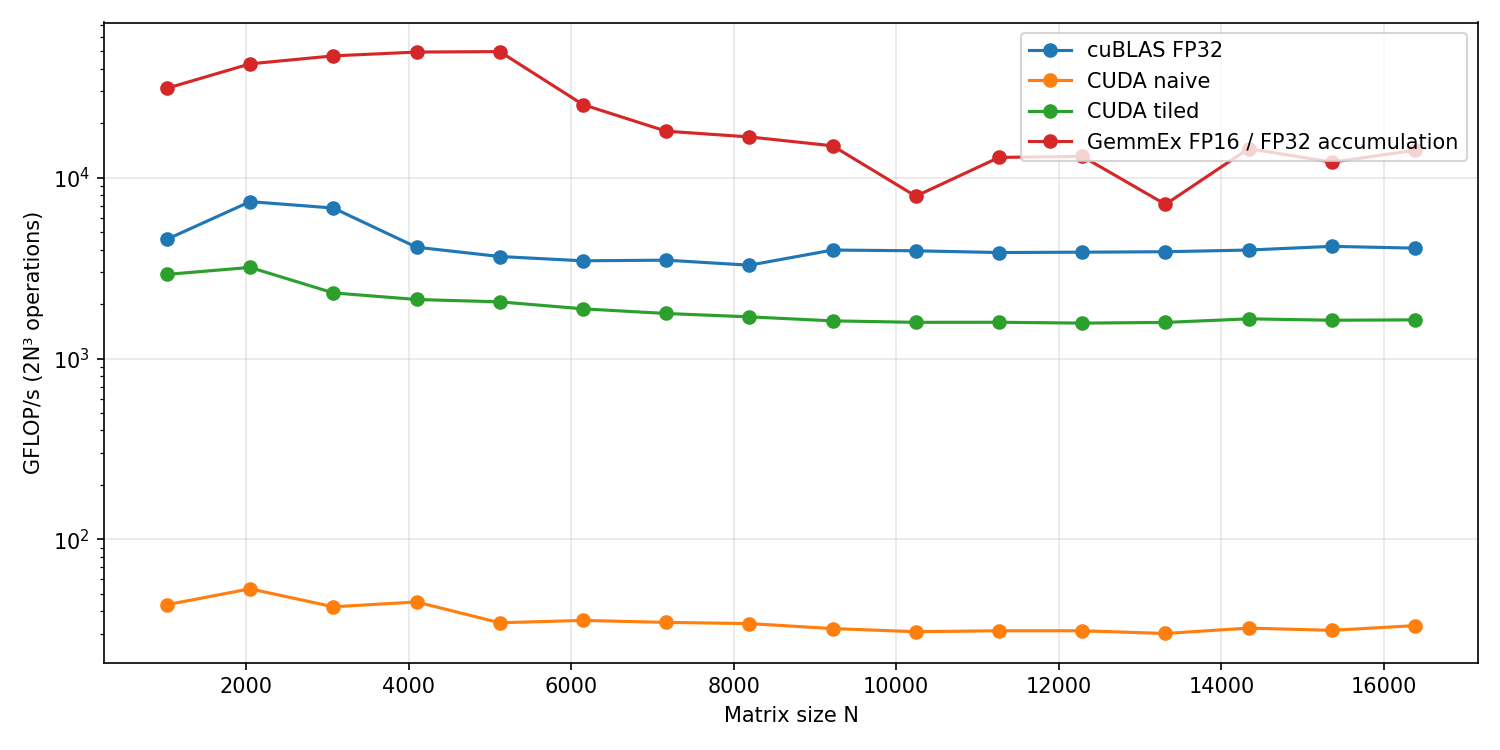
\includegraphics[width=.88\linewidth,height=53mm,keepaspectratio]{gpu_results/q38_q40_cuda.png}\par

{\small\itshape Le calcul par tuiles dépasse le kernel naïf en réutilisant les données. GemmEx, qui utilise les Tensor Cores en précision mixte, atteint le débit le plus élevé à N = 5 120.\par}\end{minipage}\par

\textbf{Conclusion sur la multiplication matricielle.} Sur CPU, à 1 920, le découpage en blocs de cache ramène le temps de 228 à 136 ms entre v5 et v6. À 9 600, le meilleur compromis mesuré est de 20 threads, avec 4,70 s et 2,40 GFLOP/J à la prise. Sur T4, à 4 096, le passage du kernel naïf au kernel par tuiles réduit le temps de 3,05 s à 64,8 ms. Dans les deux cas, réutiliser les données améliore le débit.

\clearpage

\section*{\sffamily Partie 2 — Reconnaître les chats et les chiens}

Les réseaux sont entraînés avec CIANNA pour distinguer les chats des chiens sur les photos du jeu ASIRRA. Chaque modèle est évalué sur les mêmes 2 048 images. Le but est de classer correctement le plus d’images possible et de traiter le lot entier \textbf{en moins de 300 ms sur le T4}. Sur le CPU de la salle, la limite est de 5 s.

\begin{center}\small\setlength{\tabcolsep}{3pt}\renewcommand{\arraystretch}{1.16}

\begin{tabular}{>{\raggedright\arraybackslash}p{\dimexpr 0.130\linewidth-8\tabcolsep*130/1000\relax}>{\raggedright\arraybackslash}p{\dimexpr 0.390\linewidth-8\tabcolsep*390/1000\relax}>{\raggedright\arraybackslash}p{\dimexpr 0.300\linewidth-8\tabcolsep*300/1000\relax}>{\raggedright\arraybackslash}p{\dimexpr 0.180\linewidth-8\tabcolsep*180/1000\relax}}\toprule

\textbf{Essai} & \textbf{Idée testée} & \textbf{Images bien classées} & \textbf{Inférence}\\ \midrule

1 · CPU (modèle du cours) & Images 64 × 64, deux convolutions puis trois couches denses & 83,89 \% à 500 itérations & 0,70 s\\

2 · CPU & Cinq convolutions, augmentations plus fortes et dropout réduit & \textbf{92,92 \%} à 500 & 3,63 s\\

3 · CPU & Plus de convolutions sur de petites cartes, moyenne globale et aucune couche dense & \textbf{90,48 \% au checkpoint 100}, entraînement arrêté & 2,70 s\\

4 · T4 & Images 96 × 96, première convolution de stride 2, entraînement et inférence en précision mixte & \textbf{89,70 \% à 150} en validation, \textbf{50,00 \% à 500} & \textbf{154,5 ms} au checkpoint 500\\

5 · T4 & Même architecture, entraînement FP32, inférence en précision mixte et sauvegarde du meilleur checkpoint & \textbf{94,29 \%} au meilleur checkpoint (500), après \textbf{15,09 min} & \textbf{136,1 ms}\\

6 · T4 & Images 128 × 128 au lieu de 96 × 96, architecture et entraînement de la config 5 & \textbf{95,56 \%} au checkpoint 450 (500 itérations en \textbf{17,90 min}) & \textbf{244,9 ms}\\

\bottomrule\end{tabular}\end{center}

\subsection*{\sffamily Pourquoi ces configurations ?}

\textbf{Config 1 — référence fournie par le cours.} Ce modèle sert de point de comparaison pour les essais suivants sur CPU. Entre les itérations 200 et 500, la perte d’entraînement baisse de 0,420 à 0,314. Sur la même période, la perte de validation passe de 0,401 à 0,413 et la précision de 83,30 \% à 83,89 \%. Le réseau continue donc à mieux reconnaître les images déjà vues, avec peu de gain sur les autres. Ce décalage motive les augmentations de la config 2. L’inférence prend seulement 0,70 s sur les 5 s disponibles. Il reste donc du temps pour extraire davantage de motifs dans les images.

\textbf{Config 2 — mieux exploiter les mêmes images.} Passer de deux à cinq convolutions permet de combiner des motifs simples en formes plus complexes. Les variations de couleur, d’angle et d’échelle visent à mieux reconnaître un animal quand la photo change. Le dropout des deux couches denses passe de 80 et 50 \% à 50 et 30 \% pour garder davantage de neurones actifs pendant l’apprentissage. Entre les itérations 200 et 500, la précision en validation progresse encore de 90,43 \% à 92,92 \%. Le gain final sur la config 1 atteint 9,03 points, mais l’inférence passe de 0,70 à 3,63 s. Ce coût motive la recherche des couches les plus lentes dans l’essai suivant. Plusieurs réglages ayant changé ensemble, leur contribution individuelle reste inconnue.

\textbf{Config 3 — déplacer le calcul vers les petites cartes.} Dans la config 2, la deuxième convolution à pleine résolution représente environ 42 \% du temps des couches. Avancer le premier pooling réduit le nombre de positions à traiter par les convolutions suivantes. En sortie, deux cartes donnent chacune un score par position, pour « chat » ou « chien ». La moyenne de chaque carte fournit le score de la classe sans couche dense. L’inférence descend à 2,70 s. Après 409 600 images vues, la config 3 atteint 90,48 \% contre 87,21 \% pour la 2. Entre 50 et 100, sa perte de validation descend encore de 0,346 à 0,255. L’essai est arrêté en pleine progression. Ces résultats justifient de réutiliser la tête sans couche dense sur T4, mais son score à 500 reste inconnu.

\textbf{Config 4 — garder plus de détails sur T4.} Le passage sur T4 permet de tester des images de 96 × 96. Pour viser 300 ms, la première convolution avance de deux pixels à la fois et produit directement des cartes de 48 × 48. Le calcul utilise la précision mixte. Le modèle atteint 89,70 \% à l’itération 150. L’instabilité apparaît ensuite dans les pertes. Aux itérations 250, 300 et 350, la perte moyenne d’entraînement passe de 0,53 à 0,71 puis revient à 0,53. La perte de validation oscille dans le même sens (0,52, puis 0,64 et 0,57). À l’itération 400, les deux pertes bondissent à 10,92 et 13,82. Le réseau classe alors toutes les images comme « chat » et tombe à 50 \% de bonnes réponses. Comme l’entraînement se dégrade lui aussi, ces mesures suggèrent une instabilité de l’apprentissage.

\textbf{Config 5 — tester la stabilité à architecture identique.} L’entraînement passe en FP32 pour réduire les erreurs d’arrondi. L’inférence garde la précision mixte pour rester rapide. Comparer les modèles tous les 50 tours et sauvegarder le meilleur permet aussi de récupérer les poids précédant une éventuelle chute. La précision en validation recule de 91,50 \% à 89,40 \% entre les itérations 150 et 200, puis remonte à 92,48 \% dès 250. À 500, la perte de validation descend à 0,173 et la précision atteint 94,29 \%. La baisse à 200 était donc passagère. Le résultat est compatible avec un entraînement plus stable en FP32, même si la cause exacte de la chute précédente reste inconnue.

\textbf{Config 6 — utiliser la marge de temps pour augmenter la résolution.} À 136,1 ms, la config 5 dispose encore de 163,9 ms avant la limite. Passer de 96 × 96 à 128 × 128 conserve davantage de détails de l’image d’origine avec les mêmes couches et les mêmes réglages d’entraînement. À 50 itérations, la config 6 est derrière la 5 (83,79 \% contre 86,18 \%). À 200, elle passe devant (93,60 \% contre 89,40 \%). Juger la résolution sur le premier checkpoint aurait donc conduit au choix inverse. La précision atteint 95,56 \% à l’itération 450 puis 95,51 \% à 500. Cela représente une seule image bien classée de moins sur 2 048. Le checkpoint 450 est donc retenu, mais cet écart donne peu d’indices de surapprentissage marqué.

\textbf{Deux essais possibles à partir de la config 6.} Pour la config 7, les rotations et les changements d’échelle seraient appliqués à 60 \% des images d’entraînement au lieu de 30 \%. L’objectif serait de mieux reconnaître l’animal quand son orientation ou son cadrage change, sans alourdir l’inférence. La config 8 garderait les augmentations à 30 \% et réduirait uniquement le taux d’apprentissage maximal de 0,0003 à 0,00015. Comparer la précision aux mêmes itérations montrerait si ces mises à jour plus petites améliorent le résultat ou ralentissent simplement l’apprentissage.

\textbf{Conclusion sur le CNN.} Le modèle retenu est la \textbf{config 6 au checkpoint 450}. Passer de 96 × 96 à 128 × 128 donne un gain de \textbf{1,27 point} par rapport à la config 5 pour \textbf{108,8 ms} de plus. Ce checkpoint atteint \textbf{95,56 \% de bonnes prédictions sur 2 048 images en 244,9 ms}, avec \textbf{55,1 ms de marge} sur le T4.

Les poids du modèle retenu à l’itération 450 n’ont pas été conservés.

\section*{\sffamily Annexe — Configuration 6 sur T4}

Le réseau CIANNA prend en entrée des images de 128 × 128 pixels. Ses sept convolutions produisent deux cartes, une pour les chats et une pour les chiens. La moyenne de chaque carte donne le score de la classe, sans couche dense.

L’entraînement dure 500 itérations en FP32 avec RMSProp, par lots de 32. Les augmentations font varier la couleur, l’orientation et le cadrage des images. Le modèle retenu est celui qui obtient le meilleur score de validation. L’inférence utilise la précision mixte, par lots de 128.

\textbf{Notebook joint} · \texttt{partie2/config6\_T4.ipynb}. Le notebook prépare les données, entraîne le réseau et mesure le temps d’inférence sur les 2 048 images.

\end{document}
